	\section{Is less missing data always better?}
		\subsection{Impact of mising validation data}
\todo{Include graphs to show the linear evolution of the loss (increasing and decreasing)}
		\subsection{Impact of missing train data}
%When estimating a model parameter, we generally want as little missing data as possible
%Especially, when the missing data pattern is MCAR and we have lots of complete cases, it is tempting to use just them
%However, it is possible that we really need to have the same MD pattern for train and validation (real-world data), as illustrated by empirical results: with mean imputation, the best predicition is when  there  is the same amount in both sets!
When performing an analysis, it is intuitive that we should limit the amount of missing data as much as possible, since missing data pollutes our estimates.

In particular, if the missing data is MCAR --- and so the complete cases have exactly the same distribution as those with missing data ---, and we have a large enough dataset with many complete cases (as in the Traumabase), it is tempting to use only those complete cases to learn our model. Even in a context where we are training for prediction, and the real-world data will have some missing values we need to handle, it seems that we can use complete cases in the training data to learn both our prediction and imputation parameters as accurately as possible and then use those to predict the new data at best.

However, it may not be so: when imputing missing data, we do not recover the exact initial data. What if these errors change the structure of the dataset enough that a different parameter (possibly different from the one that generated the data) can yield better predictions? In that case, learning our model without any missing data may yield the true parameter but still not be optimal for prediction.

We investigated this on some simulated data by adding a fixed proportion of missing values to the validation data (mimicking the real-world data) and varying the amount of missing data in the training set:

\begin{algorithm}[H]
	\caption{Impact of missing data}
	\hspace*{\algorithmicindent} \textbf{Input:} $\pi_V, m$  \\
	\hspace*{\algorithmicindent} \textbf{Input:} $L_1, \ldots L_m$  \\
	\begin{algorithmic}[1]
		\State $X \sim \mathcal{N}(\mu,\Sigma)$
		\State $y \leftarrow X \beta + \epsilon$ \Comment Where $\epsilon$ is a normal noise factor
		\State $X_A, X_V, y_A, y_V \leftarrow$ Random CV split of $X,y$
		\For{$\pi_A \in [0, \frac{1}{m}, \ldots \frac{m-1}{m}]$}
			\State Add proportion $\pi_A$ of MCAR missing data to $X_A$
			\State Add proportion $\pi_VA$ of MCAR missing data to $X_V$
			\State Impute $\hat{X}_A$ and $\hat{X}_V$ using $\mu_A$ the observed mean of $X_A$
			\State Compute $\hat{\beta}_A$ by linear regression on $\hat{X}_A, y_A$
			\State Predict $\hat{y}_V = \hat{X}_V \hat{\beta}_A$
			\State $L_i \leftarrow L(\hat{y}_V, y_V)$
		\EndFor
	\end{algorithmic}
\end{algorithm}

with $\Sigma = (1-\rho) I_p + \rho \mathbbm{1}$ (same correlation between all variables) and $\beta=(1,\ldots,1)$. The results are shown in Fig.\ref{fig.miss_impact3_simu} for $\rho=0.9, \pi_V=0.4$.

\begin{figure}[H]
	\centering
   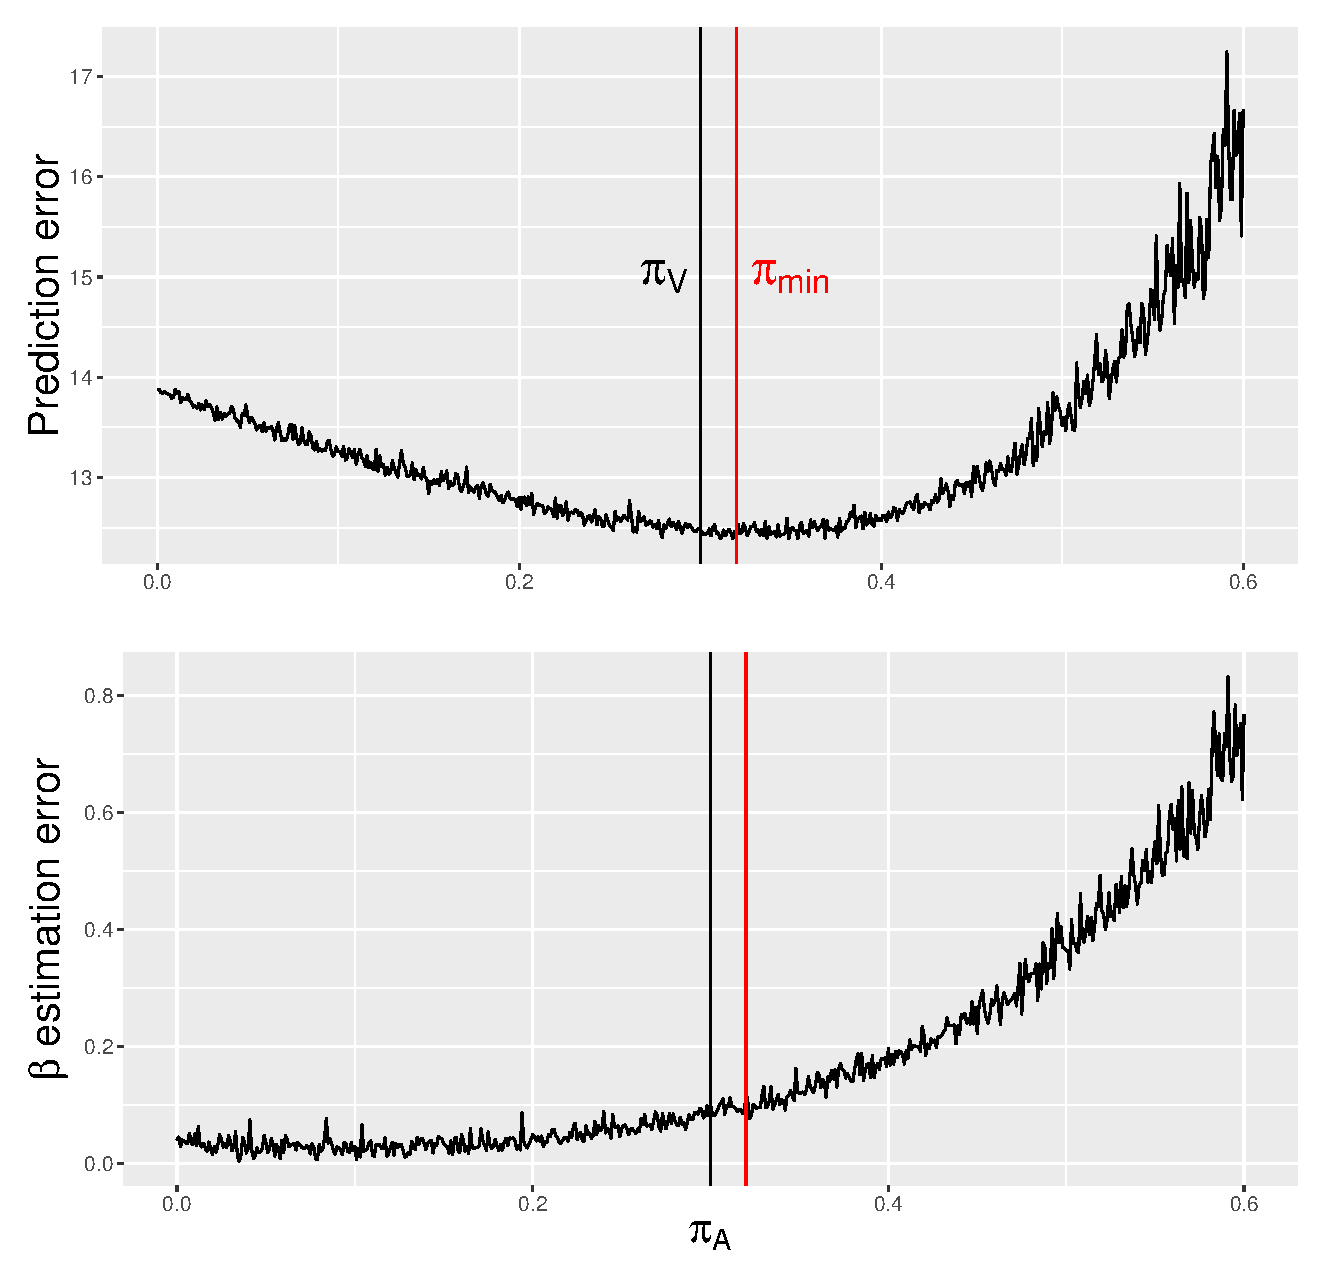
\includegraphics[scale=0.4]{Resources/miss_impact3_simu}
   \caption{Prediction and parameter estimation errors depending on train missing data proportion $\pi_A$}
   \label{fig.miss_impact3_simu}
\end{figure}

What we can see here is that when the training dataset is fully observed while the validation has missing data, the prediction error is \emph{higher} than in the same situation with missing data in the training set as well. More precisely, the best prediction is achieved when both datasets have roughly the same amount of missing data.

It is not clear how general this result is. The same trend was visible on the real-world Abalone dataset, and on simulation through a range of parameters. However, we could obtain it \emph{only when using mean imputation}: with more elaborate imputation methods it did not show.

 In any case, this warrants caution when doing cross-validation with missing data: while reducing the amount of missing data in our records is a worthy endeavour --- e.g. by deleting incomplete cases ---, it is possible that it will only be useful if the real-world (or validation) data also has less missing data as a result --- e.g., improving the data-collection process. Additionally, just as it is important to ensure that the distribution of the data is stable between training and application --- no temporal trend in the data ---, the same should be done about the missing-data pattern.
	\section{Using $y$ in the imputation}
	\section{Multiple imputation}
		\subsection{Prediction intervals}
		\subsection{Point estimate}